\section{Implementation}%
\label{sec:implementation}
We have implemented a full-featured prototype of HyperPS.


\subsection{HyperPS Space}%
\label{sub:hyperps_space}
% In this paper, HyperPS creates a delicate kernel-level secure and isolated execution space, called HyperPS Space, to inherit privileges of managing physical memory that originally belonged to the compromised hypervisor.
% HyperPS does not rely on a higher privileged layer or any special hardwares.
\iffalse 

实现了虚拟机的隔离主要通过保护和隔离EPT和虚拟机内存来完成,主要完成4部分,1)实现vm-mark表,将VM与EPT进行绑定确保各虚拟机只能访问自己的EPT。2)hyperps剥离了EPT相关的所有访问函数,保证ept表的安全访问。以防被恶意更改。3)页分配时实现page-mark表,来标注page唯一的属主vm,保证vm-ept-page的一致性。在页分配时验证页的属主,空页绑定页与vm,非空页验证属主,以免页被重新分配。4)页释放时清除页内容。如果原vm的内容页在释放时未被清除,当该页再次分配给其余虚拟机时,其上的内容可能被恶意虚拟机读取而泄露数据。

We propose ept isolation and vm isolation by preventing ept access and released vm page access , following the steps. 1) Guarantee the consistency of vm and ept. Making vm-ept mark table to ensure EPT isolation and one VM only access own corresponding EPT. 2) Strips ept access privilege. Strips all access functions related to EPT to ensure safe access and to ept and prevent malicious changes. 3) Page-mark table. The page-mark table is created marking the unique owner vm of the page during page allocation. So the consistency of vm-ept-page can ensure ept isolation and vm isolation, one vm can only access own ept and own pages. During page allocation, the owner of the page is verified, empty pages are bound to the vm directly, and the allocated page is discarded to prevent the page from being remapped. 4)Clear page content when released. If the content page of the original vm is not cleared after being released, after allocated to other virtual machines again, the content on the page may be read by a malicious virtual machine so that privacy data may be leaked.
 
It is important to ensure EPT isolation and one VM only access own corresponding EPT. To ensure one EPT for one VM, HyperPS creates the VM-Mark structure stored in HyperPS World as Table I described. It records VMID, EPTID, EPT Address and binds them together. VMID is created when the VM is created. EPTID and EPT Address is recorded as long as the EPT of current VM is created. This table is destroy once the VM is shutdown or destroyed.
 
Vm-ept mark table is hidden in hyperps world. all access functions for EPT address must be executed in hyperps world. When EPT is created, use the hash function to construct the ID number of the ept according to the ept address, bind it to the current VMID as a structure, the relationship between VM and EPT is established. Other access functions of EPT, such as reading and writing,updating will be executed  in hyperps wolrd for safety.
Stripping EPT's access capability can prevent attackers from tampering with EPT. When 
\fi


In this paper, we create a delicate kernel-level trusted execution environment, called HyperPS Space, to inherit privileges of managing physical memory that originally belonged to the compromised hypervisor. 
The HyperPS Space achieves isolation and secure context switching without relying on a higher privileged layer or any special hardwares. 
% As shown in Figure \ref{fig:address}, we create the HyperPS Space by using two set of page tables.
% describes the address layout of HyperPS.

\iffalse
在创建的时候,要讲明白为什么是Hypervisor的情况下,要从hostos出发。
首先是创建,创建完成之后再写如何保证隔离的 即prohibit the kernel from modifying the momory layout or access permission of the system.
\fi
% does not rely on a higher privileged layer or any special hardwares.


\subsubsection{The Creation of HyperPS Space}%
\label{ssub:hyperps_space_creation}

\iffalse
% Figure \ref{fig:address} describes the address layout of HyperPS.
这段要说明为什么要在hostOS上使用两套页表的方法创建同层隔离的空间。
当hostos已经不可信的时候,我们需要一个全新的TEE用于host我们的保护工具。在这篇文章中,我们采用了同层隔离的方式来创建我们的TEE。
我们通过两步创建我们的space,首先是在什么地方创建,其次是保证其隔离性。
% 一个合格的TEE应该
\fi

In our prototype, we create the HyperPS Space by using two set of page tables.  
Figure \ref{fig:address} describes the address layout of HyperPS. 
\begin{figure}[htpb]
    \centering
    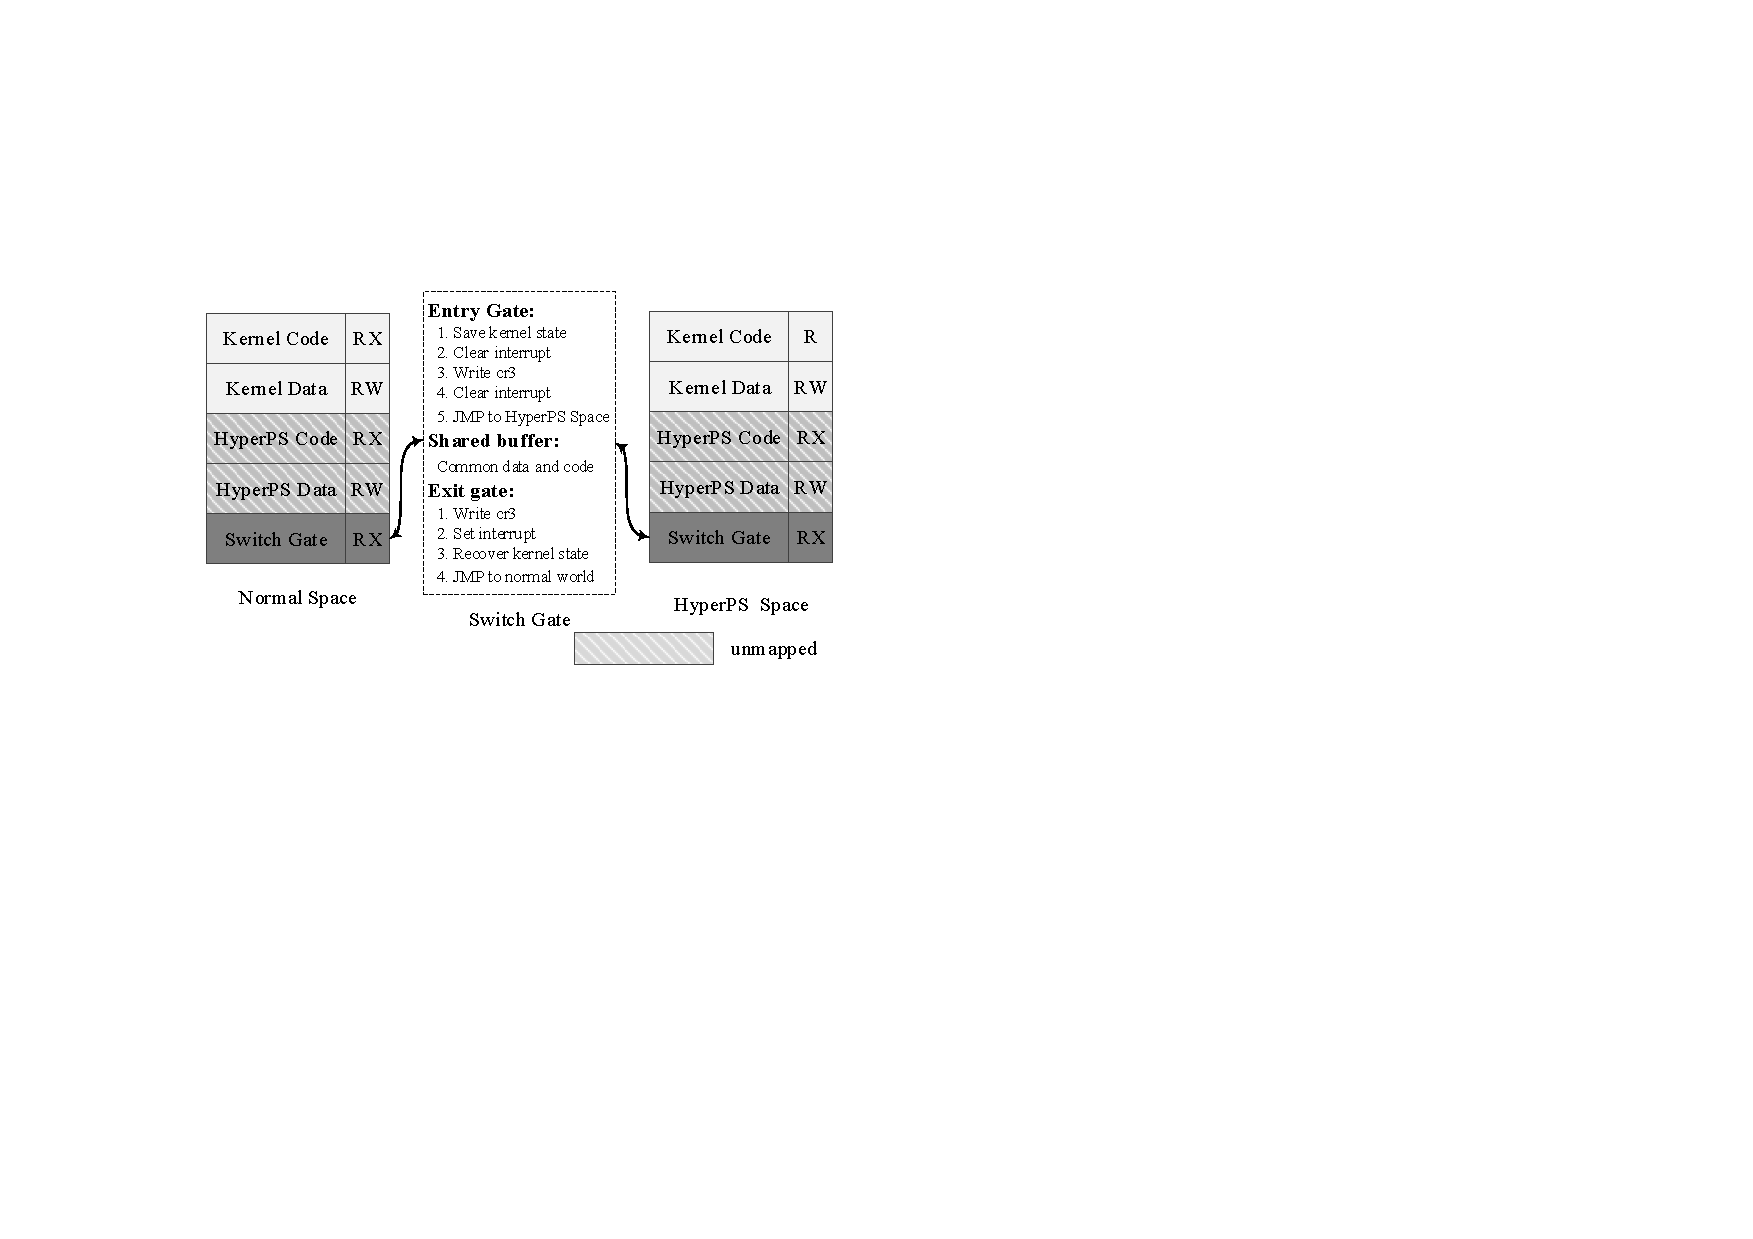
\includegraphics[width=0.8\linewidth]{IMG/address.pdf}
    \caption{Address layout of HyperPS}%
    \label{fig:address}
\end{figure}


% However,
% HyperPS Space的创建并不能在kernel boot阶段,因为此时,内核需要
% hostos的kernel并不能在boot的时候就直接完成两套页表的建立。
% As shown in this figure, HyperPS has to load itself into memory at first.
As shown in this figure, at the initialization stage, HyperPS has to load itself into memory firstly before it got executed. 
At this stage, all resources are managed by the Hostos kernel, HyperPS needs to request enormous number of memory allocation from the Hostos. These memory are used to hold HyperPS data and security tools that inherit compromised hypervisor's privileges of managing physical memory. 
In our prototype, we do not guarantee that all allocated memories are continuous in physical memory. 
Secondly, HyperPS creates a new page table that has already excluded the HyperPS Space. As shown in Figure \ref{fig:address}, this dedicated page table is placed in the normal space and accessed by the compromised HostOS kernel. 
Because all page table entries that are relative to HyperPS Space have been removed from that dedicated page table, 
% normal memory access beyond the HyperPS Space can not visit memory regions of HyperPS Space.
memory regions used by HyperPS are carved out of the memory reanges accessible to the HostOS kernel. 
% Thirdly, HyperPS will set a new GDT, IDT and stack for itself.
At last, HyperPS returns execution back to the normal space by loading the address of the dedicated page table into the control register CR3. 

On the execution of the three steps mentioned above, HyperPS has established an execution environment. 
However, at this time, this execution environment does not have the conditions for isolation and security, since the kernel can still modify this memory layout or access permission. 


\subsubsection{The Isolation of HyperPS Space}%
\label{ssub:the_isolation_of_hyperps_space}
% HyperPS has created a protected virtual address space.
HyperPS has to guarantee that memory regions used by HyperPS are carved out of the memory ranges accessible to the kernel.
In oder to achieve the isolation of the HyperPS Space, HyperPS restricts the compromised HostOS kernel access to this space. 
% To protect HyperPS Space, firstly, we deprive the write permission to whole kernel page tables,
Firstly, we remove write permissions to whole kernel page tables, so that the HostOS kernel can not modify the dedicated kernel page table in the Normal Space. In out prototype, the HostOS kernel can still navigate and examine page table entries, while write operations through legitimate page table management functions and macros are hooked and redirected into HyperPS Space. 
Meanwhile, direct write operations to the dedicated kernel page table will trigger error. 
% In our prototype, all page table write operations are completed inside the HyperPS Space.
% any modification operation will
% to
% navigation and examination of page table entries
% so that they are exclusively writable to HyperPS in the HyperPS Space.
% To protect HyperPS Space, write permission to HostOS kernel page tables
Secondly, as mentioned above, HyperPS removed all page table management functions and macros and replaces them with hooks that jump to HyperPS Space, so that any modification to the dedicated kernel page table in the normal space will be redirected to HyperPS Space. 
For example, \verb|native_set_pte()| is the funtion that acutally implements PTE operations. Other PTE operation functions such as \verb|set_pte()| and \verb|native_set_pte_atomic()| all invoke the \verb|native_set_pte()| function to accomplish their implementation. 
% implement their
% will implement their operation by invoking this function.
In our prototype, HyperPS hooks all these final and elemental page table management functions and macros.
% For example, we hooked \verb|native_set_pte|, \verb|native_set_pmd| and \verb|do_page_fault|
HyperPS makes sure that the HostOS kernel can neither tamper the virtual memory permissions of the HyperPS Space, nor can it establish new mapping relationship to the physical memory frames related to the HyperPS Space. 
% For example,
In another word, the HostOS kernel page table are exclusively writable to HyperPS only. 
Lastly, HyperPS deprives the HostOS kernel from executing certain Control-Register-Relative functions so that it cannot direct the CPU to use alternative page tables other than the dedicated one we put in the normal space. 
% In this paper, HyperPS instrumented the kernel code to remove certain Control-Register-Relative functions.
For example, \verb|native_write_cr3()| is written with inline assembly language to load page table's physical address into the register CR3. 
HyperPS instrumented this function to prevnet the adversary from using a unverified page table. 
% HyperPS instrumented the function \verb|native_write_cr3| to prevent the adversary from using a unverified page table.
HyperPS also intercept the accessing operation to Control Register: CR0 to prevent the adversary from disabling WP protection mechanism.
Actually, HyperPS hooked \verb|native_write_cr0()|, \verb|native_write_cr2()|, \verb|native_write_cr3()|, and \verb|native_write_cr4()| to HyperPS Space.
% redirect the execution to HyperPS Space.
% , such as the ones that change the vulue of CR0, CR3, and CR4.
By enforcing these three steps, the HostOS kernel running in the normal space is neither allowed to modify the dedicated host kernel page table nor change the control register configurations to use unverified page tables. 
As a result, the HostOS kernel cannot violate the isolation provided to HyperPS, since HyperPS deprives the HostOS kernel privileges of access to control registers and page tables and retains these privileges in the HyperPS Space.

% As a result, the HostOS kernel cannot violate the isolation provided to HyperPS, while HyperPS retains the exclusive access to control the control registers and page tables in the HyperPS Space.
% which
% is deprived the privileges of accessing to control registers and page tables in the HyperPS Space.
% retains the exclusive access to control the control registers and page tables in the HyperPS Space.



\iffalse
HyperPS makes sure that the HostOS kernel cannot modify any of the dedicated kernel page table to tamper the virtual memory access permissions of HyperPS Space. 

memory region used by HyperPS are carved out of the memory ranges accessible to the kernel.

In another word, the HostOS kernel page table are exclusively writable to HyperPS only. 


HyperPS will check 
so that the HostOS kernel is not allowed to change any ken
% Secondly, we also hook all page table management functions and macros to HyperPS Space, so that

. For example, we instrumented 

all page table functions 

这里HyperPS分为两步实现保护,一方面限制所有PT访问的函数。另外一方面限制CR3函数 

It starts by instrumenting the kernel code to remove certain MMU control instructions. such as the ones that change the location of memory tranlation tables. 
SEKK also monitor memory layout changes to guarantee that no other unverified privileged code is allowed to execute. 

hook的函数:
pte pme pagefualt 
vmcs read write clear 
pfn modify map 
clean page modify 
ksm page modify
\fi


\iffalse
下面的这部分内容应该是保护的内容,涉及的是EPT和缺页中断的处理,不应该是地址空间创建这部分内容。
在QEMU-KVM架构下,一台虚拟机的memory space同时受宿主机的page table和EPT两套页表管理。
% 在non-root模式下,
对于宿主机而言,虚拟机就是一个qemu进程,这个与其他的普通进程没有区别,宿主机通过传统的页表管理qemu所需要的所有地址空间。hostOS负责实际分配给该虚拟机的所有物理页框。
当EPT enable的时候,
在root模式下,EPT负责将qemu进程的

在QEMU-KVM架构下,以HostOS 视角看,整个虚拟机即为一个QEMU进程,EPT用于管理已经分配给QMEU进程中的物理页。
Traditional page tables continue to be reponsible for FVA-GPA, while EPT is responsible for GPA-HPA.
\fi

\iffalse
As shown in the Figure \ref{fig:address}, HyperPS creates the delicate kernel-level secure and isolated execution space by using two sets of page tables. 
On the left side of Figure \ref{fig:address}, the normal page table contains code and data of the HostOS kernel world. However, page table entries about the HyperPS Space has been removed from this table. %The attacker can not subvert the HyperPS Space 
Because all corresponding page table entries have been removed, the attacker can not find out in which memory the HyperPS Space locates, let alone subvert programs in the HyperPS Space. 
As shown in the Figure \ref{fig:address}, The Switch Gate is the only way that can perform the context switch from the Normal Space (the original hypervisor space) to the HyperPS Space.
On the other side of Figure \ref{fig:address}, HyperPS safeguard the integral page tables which contain both the kernel code, data and the HyperPS code, data. Besides, HyperPS removed the execution permission of all kernel code to prevent unauthorized code execution.
\fi

\subsection{Switch Gate}
Switch Gate is designed to allow secure switching between HyperPS Space and the Normal Space, and it is the only interface between the Normal Space and the HyperPS Space. In this paper, HyperPS adopts a technique similar to the one presented in SKEE \ref{Azab2016SKEE}. Our Switch Gate can achieve atomic, deterministic and exclusive too.
% Switch Gate is the only interface between the Normal Space and the HyperPS Space. HyperPS adopts a technique similar to the one presented in SKEE \ref{Azab2016SKEE}. In this paper, our Switch Gate is designed to allow secure switching between HyperPS Space and the Normal Space. Our Switch Gate is designed to be atomic, deterministic and exclusive too.
As shown in the middle block of Figure \ref{fig:address}, the Switch Gate mainly consists of three parts: the Entry Gate, the Exit Gate and the Shared Buffer. 
The Entry Gate provides the only entrance for HyperPS Space. The Entry Gate will save the HostOS kernel state into the Shared Buffer first. Secondly, it will clear and disable interrupts. Interrupts could enable the compromised HostOS kernel crash the atomic execution of Switch Gate. 
Then HyperPS will enter the HyperPS Space by loading the page table used by HyperPS Space into register Cr3. 
% load the page table used by HyperPS Space into register CR3.
The address of this page table is visible to HostOS kernel, however, as mentioned above, because all page table management functions and control register management function have been hooked by HyperPS, the compromised HostOS kernel cannot subvert the HyperPS Space by using unverified page tables. 
Lastly, we clear interrupts with \verb|CLI| instruction again before we execute any instruction in the HyperPS Space. 
% divert execution into HyperPS Space.
The Exit Gate is the only interface that can divert execution back to Normal Space. It can only be invoked by HyperPS from the HyperPS Space. 
On recieving the invocation to Exit Gate, 
HyperPS will load the dedicated HostOS kernel page table into register CR3, recovere interrupts, and recover saved kernel state. 
The Shared Buffer contains data and code shared by the Normal Space and the HyperPS Space. For example, as mentioned above, the entrance address of HyperPS Space and the return address to the Normal Space are stored in this buffer. HyperPS also stores the saved kernel state in this buffer. 
% In our prototype, we mapped the Switch Gate at the same place in both Normal Space and the HyperPS Space.

However, TLB becomes a subtle issue in the implementation of our Switch Gate. TLB is a special cache used to keep track of recently used PTE transactions.
Given a virtual address, the processor wll first examine the TLB if a PTE is present (TLB hit). If a match is found in the TLB, the processor retrieves the corresponding physical memory frame number from TLB directly. If the mapping is not cached by the TLB, the processor retrieves the physical memory page number from page table residing in the main memory and updates the new PTE into TLB. Thus, we need to flush TLB after we update both dedicated HostOS kernel page table and the page table used by HyperPS. 
In our prototype, we borrowed the idea in SecPod that clears the global bits in both the dedicated HostOS kernel page table and the HyperPS Space page table. By doing so, the TLB will always contain fresh address mappings after invoking the function\verb|flush_tlb_all()|.
% n HyperPS Space and

% there is one subtle issue in the implementation of the Switch Gate

% The switch gate is mapped at the same place in the Normal Space and the HyperPS Space, because the switch gate code must be called by the two worlds before and after switching. Of course, the entrance address must be protected after switching to HyperPS Space in case that a attacker accesses HyperPS Space causally after trusted boot. Protection to Switch Gate will be illustrated in the Section \ref{sec:securityforhyperps}.



% The shared buffer contains common data and code in Normal Space and the HyperPS Space. Common code is switch code, common data is entrance address to HyperPS Space and return address to the Normal World.
% On invoking Exit Gate,
% jump into
%  before
% address of page table

% HyperPS achieves the atomic secure switching
% Disabling interrupts
% 为什么要屏蔽中断,这里要说清除。

\iffalse
In the middle of Figure \ref{fig:address}, the switch gate includes entry/exit gate and shared buffer. Entry gate provides the only entrance to HyperPS Space and the exit gate provides the address for returning to the Normal Space. The shared buffer contains common data and code in Normal Space and the HyperPS Space. Common code is switch code, common data is entrance address to HyperPS Space and return address to the Normal World. The switch gate is mapped at the same place in the Normal Space and the HyperPS Space, because the switch gate code must be called by the two worlds before and after switching. Of course, the entrance address must be protected after switching to HyperPS Space in case that a attacker accesses HyperPS Space causally after trusted boot. Protection to Switch Gate will be illustrated in the Section \ref{sec:securityforhyperps}.
%添加Section的引用
\fi

\iffalse
except for that of HyperMI World. This can prevent compromised hypervisor from breaking the integrity of HyperMI World. Programs running in normal world can not access data in HyperMI World. On the right of Figure \ref{fig2}, all address is mapped in HyperMI page table.

 We use two isolated address spaces based on two sets of page tables to achieve isolation of HyperMI World.
Figure \ref{fig2} describes the address space layout of two worlds through two sets of page table, the normal page table and HyperMI page table. On the left of Figure \ref{fig2}, the normal page table contains code and data of the normal world except for that of HyperMI World. This can prevent compromised hypervisor from breaking the integrity of HyperMI World. Programs running in normal world can not access data in HyperMI World. On the right of Figure \ref{fig2}, all address is mapped in HyperMI page table.
HyperMI code remains executable and HyperMI data remains writable. What's the most important, kernel code is forbid to execute when HyperMI World is active, so that it can not attack HyperMI World.

\textbf{Creating Switch Gate}
In the middle of Figure \ref{fig2}, the switch gate includes entry/exit gate and shared buffer. Entry gate provides the only entrance to HyperMI World and the exit gate provides the address for returning to the normal world. The shared buffer contains common data and code in normal world and HyperMI World. Common code is switch code, common data is entrance address to HyperMI World and return address to the normal world. The switch gate is mapped at the same place in the normal world and HyperMI World because the switch gate code must be called by the two worlds before and after switching. Of course, the entrance address must be protected after switching to HyperMI World in case that a attacker accesses HyperMI World causally after trusted boot. This is introduced in section \ref{SG}.
\fi



\iffalse
下面的这部分内容应该是保护的内容,涉及的是EPT和缺页中断的处理,不应该是地址空间创建这部分内容。
在QEMU-KVM架构下,一台虚拟机的memory space同时受宿主机的page table和EPT两套页表管理。
% 在non-root模式下,
对于宿主机而言,虚拟机就是一个qemu进程,这个与其他的普通进程没有区别,宿主机通过传统的页表管理qemu所需要的所有地址空间。hostOS负责实际分配给该虚拟机的所有物理页框。
当EPT enable的时候,
在root模式下,EPT负责将qemu进程的

在QEMU-KVM架构下,以HostOS 视角看,整个虚拟机即为一个QEMU进程,EPT用于管理已经分配给QMEU进程中的物理页。
Traditional page tables continue to be reponsible for FVA-GPA, while EPT is responsible for GPA-HPA.
\fi


\iffalse 

实现了虚拟机的隔离主要通过保护和隔离EPT和虚拟机内存来完成,主要完成4部分,1)实现vm-mark表,将VM与EPT进行绑定确保各虚拟机只能访问自己的EPT。2)hyperps剥离了EPT相关的所有访问函数,保证ept表的安全访问。以防被恶意更改。3)页分配时实现page-mark表,来标注page唯一的属主vm,保证vm-ept-page的一致性。在页分配时验证页的属主,空页绑定页与vm,非空页验证属主,以免页被重新分配。4)页释放时清除页内容。如果原vm的内容页在释放时未被清除,当该页再次分配给其余虚拟机时,其上的内容可能被恶意虚拟机读取而泄露数据。

We propose ept isolation and vm isolation by preventing ept access and released vm page access , following the steps. 1) Guarantee the consistency of vm and ept. Making vm-ept mark table to ensure EPT isolation and one VM only access own corresponding EPT. 2) Strips ept access privilege. Strips all access functions related to EPT to ensure safe access and to ept and prevent malicious changes. 3) Page-mark table. The page-mark table is created marking the unique owner vm of the page during page allocation. So the consistency of vm-ept-page can ensure ept isolation and vm isolation, one vm can only access own ept and own pages. During page allocation, the owner of the page is verified, empty pages are bound to the vm directly, and the allocated page is discarded to prevent the page from being remapped. 4)Clear page content when released. If the content page of the original vm is not cleared after being released, after allocated to other virtual machines again, the content on the page may be read by a malicious virtual machine so that privacy data may be leaked.
 
It is important to ensure EPT isolation and one VM only access own corresponding EPT. To ensure one EPT for one VM, HyperPS creates the VM-Mark structure stored in HyperPS World as Table I described. It records VMID, EPTID, EPT Address and binds them together. VMID is created when the VM is created. EPTID and EPT Address is recorded as long as the EPT of current VM is created. This table is destroy once the VM is shutdown or destroyed.
 
Vm-ept mark table is hidden in hyperps world. all access functions for EPT address must be executed in hyperps world. When EPT is created, use the hash function to construct the ID number of the ept according to the ept address, bind it to the current VMID as a structure, the relationship between VM and EPT is established. Other access functions of EPT, such as reading and writing,updating will be executed  in hyperps wolrd for safety.
Stripping EPT's access capability can prevent attackers from tampering with EPT. When 
\fi




\iffalse
5.2内存所有权跟踪

   为了确保VMM和它的guest VM之间的内存隔离,CloudVisor保持了一个表来跟踪每个物理内存页的所有权。这个表中的值是这个页的所有者ID。每个VM在被引导时被分配了一个独一无二的ID。VMM的ID被固定为0。CloudVisor确保一个物理内存页只能在同一时间被分配给一个所有者。
   在系统启动过程中,所有的除了在CloudVisor中的页都被VMM拥有。当guest VM的EPT被第一次加载进处理器时,CloudVisor进入整个EPT来找到所有被映射的页。这些页被认为被分配给guest VM。CloudVisor改变这些页的所有者给guest VM,并且将它从VMM的EPT中取消映射,这样VMM就再也不够触及这些页了。当一个页从EPT中被取消映射时,页的所有者被设置成VMM,并且这个页在VMM的EPT中被重新映射。
   无论何时VMM更新guest EPT,在EPT中的一个页错误(在Intel词汇中的EPT violation)会发生。CloudVisor通过验证页的所有者来处理错误。当一个新的映射被建立时,CloudVisor确保要被映射的页属于VMM。CloudVisor将它从VMM的EPT中取消映射,并且改变页的所有者给guest VM。当一个已存在的页被取消映射时,CloudVisor加密这个页的内容,把它映射到VMM中的EPT,并且改变VMM的页所有者。CloudVisor不允许一个页被映射到相同的EPT中超过一次。为了重新映射一个页,VMM需要首先取消映射它,然后将它重新映射到新的位置

5.3合法内存存取
   CloudVisor提供的内存隔离机制确保guest VM的整个内存空间不能被VMM和management VM存取。然而,有几种情况,VMM和management VM应当被允许存取guest VM的一些内存。在这样的情况下,CloudVisor干预并且帮助这样的存取来确保只有最小化的非敏感数据被泄露。
   特权指令,比如IO指令和控制寄存器的存取会导致trap(如VM退出),这些trap会被VMM处理。在一些情况下,VMM在guest VM的内存中需要得到指令操作码来仿效它。在这样的trap中,CloudVisor取得特权操作码,并且将它提供给VMM。因为CloudVisor只允许获取被程序计数器指向的一个操作码,VMM就不能够欺骗CloudVisor来取得任意没有权利的操作码,也不能任意触发陷阱来得到操作码。
   在一次trap中,故障指令的程序计数器是一个虚拟地址,并且内存操作数也被表达成虚拟的地址。VMM需要去查询guest VM中的页表来将虚拟地址翻译成guest物理地址,然后要进一步使用EPT翻译成host物理地址。为了处理这个情况,CloudVisor短暂地允许VMM来间接地读取操作码和内存操作数对应的guest页表条目。当一个trap由特权指令的执行产生时,CloudVisor得到指令的程序计数器并且分析这个指令来获取内存操作数。CloudVisor查询guest VM中的页表来获取需要的页表条目,来翻译程序计数器和内存操作数。当VMM存取页表时,CloudVisor提供给它先前获取的页表条目。为了减少跟特权指令仿真相关联的开销,CloudVisor使用一个缓冲区来高速缓冲每个VCPU的特权指令的页表条目。
   仿效IO存取时,当VMM也需要得到guest IO的缓冲区内容。当VMM存取IO缓冲区时,一个EPT错误会发生,CloudVisor通过复制 给VMM的数据 来处理错误。确切地说,当VMM从或者向guest VM复制数据时,CloudVisor验证guest VM的缓冲区地址是一个已知的IO缓冲区,并且决定是否这个缓冲区被磁盘IO所用(部分6.1)。

\fi
















